\swiftColor
When dealing with large collections of data or several different programs, it can be troublesome to configure individual settings or to have a single script run through. Doing this on a normal programming language would require more effort, and may have trouble dealing with either larger amounts of data or is unable to speed up individual tasks. This becomes more pertinent as we use parallel computing to hasten our programs, but how do we manage several programs with larger datasets?

Swift is an implicit, "parallel", scripting language that heavily aids with these distributed tasks, allowing for several of the same or different programs to run concurrently through the Java Virtual Machine (JVM). Although it is currently not a full version, Swift has been used for several scientific programs such as protein structure prediction, glass structure modeling, and modeling climate and economics. There has also been discussion for petascale supercomputing using Swift as the parallel computing language \cite{wilde2009parallel} for future computation.

What makes Swift so powerful is its built-in support for bash, allowing different Swift applications to run bash commands. This feature allows it to run many different programs in several different programming languages, as they use bash to process them. This is important, as Swift itself can only assign variables once and is very focused on optimizing applications. But how does Swift use bash and perform these tasks?

\subsection{Language Basics}
    Swift is very similar in syntax to languages such as C and Java, but they don't have any object type or class type. Instead, they use data structures, references, and some atomic structures to define their data as well as how they use them for different Swift procedures, instructions, and external calls. \cite{website:swift-lang-user-guide}

    \subsubsection{Types}
        Swift is strongly-typed, with types being \textit{atomic} or \textit{composite}. An atomic type can be a \textit{primitive} (\texttt{int}, \texttt{string}, \texttt{float}, or \texttt{boolean}) or a \textbf{marker} type, which signifies that data for that variable is stored in a single file. As for composite types, they can either be arrays (integers or another primitive type for associative arrays) and a structure used to contain other variables.

        \begin{lstlisting}[language=swift]
// ----------------
// Atomic Types
// ----------------

// Primitives
string name = "Nick LaPosta";

// Marker Type
type image;
image photo <"lena.png">;

// ----------------
// Composite Types
// ----------------

// Arrays
string coolPeople[] = ["John"];
float[string] constants;
constants["pi"] = 3.1415926535;

// Structures
type circle {
    int radius;
    string color;
};
        \end{lstlisting}

    \subsubsection{Variables}

        Variables themselves are only single-assignment, meaning you can only write to a variable once. If the variable is not yet assigned and attempt to read has been made, the code performing the read is suspended until the variable has been written to. This is the same with arrays, except each of their elements can have one assignment.

        Arrays in this case are written in two different ways. The first way, \texttt{<valueType> arrayName[]}, represents an array of value and can access different values using an integer from 0 to the length of \texttt{arrayName}. The second method is for associative arrays which is set as \texttt{<valueType>[<keyType>] arrayName}, and where \texttt{keyType} is an instance.

    \subsubsection{Mappers}

        The marked type is probably the newest thing seen from any language. Typically, this is some file type that refers to an explicit file either generated or soon to be generated from some assignment. However, to link our marked type to some file, we must use a \textit{mapper}. Swift has several built-in mapping primivites (\textit{"mappers"}) that make a variable refer to a filename. These are used to not only obtain values, but also generate output text for later use or analysis.

        The default mapper used is the \textit{single file mapper}, which maps a single file to a dataset. As we can see, it reads a single file to map to a single file variable. This can also simply take a filename instead of defining the mapper and the filename together. \cite{website:swift-lang-user-guide}

        \begin{lstlisting}[language=swift]
file f <single_file_mapper;
        file="plot_outfile_param">;
file f <"plot_outfile_param">;
        \end{lstlisting}

        The \textit{simple mapper} is similar to the single file mapper, except it uses more file matching methods in order to find a set of files. It does this using a prefix, suffix, and pattern parameter that can be used to search for files in a directory, where the pattern matcher is based on UNIX glob. You may also set the location using the location parameter as well.
        \begin{lstlisting}[language=swift]
file f <simple_mapper;
        prefix="foo", suffix=".txt">;
        \end{lstlisting}
        When using an array of files, you can initialize them by using the padding parameter to set the number of digits used to map each file, although the default is 4. In the program below, our output files will be far00.txt, far01.txt, and far02.txt.
        \begin{lstlisting}[language=swift]
messagefile outfile[] <simple_mapper;
        prefix="far",
        suffix=".txt",
        padding=2>;

outfile[0] = greeting("hello");
outfile[1] = greeting("middle");
outfile[2] = greeting("goodbye");
        \end{lstlisting}
        We may also use structs with the simple mapper, using variable names within our struct to edit the name of our file as well. By running our example program below, our output files will be goleft.txt and goright.txt.
        \begin{lstlisting}[language=swift]
type messagefile;

type mystruct {
  messagefile left;
  messagefile right;
};

...

mystruct out <simple_mapper;
        prefix="go",
        suffix=".txt">;

out.left = greeting("hello");
out.right = greeting("goodbye");
        \end{lstlisting}

        Although the simple mapper can map components of the variable name, the \textit{filesystem mapper} maps directory contents into an array. This allows us to communicate with our data within a directory more simplistically. Similarly to our simple mapper, we define a prefix and suffix (or pattern) within a possible location for which our mapper will map to an index. Although this is useful for dealing with several datasets within our directory, the resulting array's order isn't defined.
        \begin{lstlisting}[language=swift]
file texts[] <filesys_mapper;prefix="foo",
        suffix=".txt">;
        \end{lstlisting}

        These were the original 3 mappers defined by the Swift paper in 2011 \cite{wilde2011swift}, but since then 7 new mappers have been created as part of Swift version 0.96. This includes a \textit{concurrent mapper}, which is similar to the simple mapper except used for mapping an output file containing an unique extract sequence. This is also the default mapper when none is specified.

        \begin{lstlisting}[language=swift]
file f1;
file f2 <concurrent_mapper;prefix="foo",
        suffix=".txt">;
        \end{lstlisting}

        When wanting to refer to several files directly, a \textit{fixed array mapper} or an \textit{array mapper} can be used to insert an array, or comma-separated string for the fixed array mapper, to choose specific files and in what order.

        \begin{lstlisting}[language=swift]
string s[] = [ "a.txt", "b.txt", "c.txt" ];
file f[] <array_mapper;files=s>;
file texts[] <fixed_array_mapper;
    files="file1.txt, fileB.txt,
            file3.txt">;
        \end{lstlisting}

        There is also a \textit{regular expression mapper} and \textit{structured regular expression mapper} which can use regular expression to transform one file name into another (or an array of filenames for the structured regex mapper). To do this, they use a file, a regex match to use, as well as and a transform to define the new name. This can be used with groupings, where you would define a group in the match parameter using parentheses and define it using two blackslashes and the group number. In the example below, we transform one file, then a set of files, from gifs to jpgs.

        \begin{lstlisting}[language=swift]
file s <"picture.gif">;
file f <regexp_mapper; source=s,
    match="(.*)gif",
    transform="\\1jpg">;

file s[] <filesys_mapper;
    pattern="*.gif">;
file f[] <structured_regexp_mapper;
    source=s,
    match="(.*)gif",
    transform="\\1jpg">;
        \end{lstlisting}

        Because of how common comma-separated values (CSVs) are, they have also received their own mapper. The \textit{CSV mapper} uses a file to fill in details on a struct, which then uses parameters such as whether the header exists (by default true), the number of lines to skp from the beginning (by default 0), hdelim or header delimiter (the default isn't exactly stated, but is believed to be commas), and lastly the CSV content delimiter (by default spaces, tabs, and commas). The example below shows a basic use of the mapper with a type struct.

        \begin{lstlisting}
type student {
  file name;
  file age;
  file GPA;
}

student stus[] <csv_mapper;
    file="stu_list.txt">;
        \end{lstlisting}

    Lastly, there is the \textit{external mapper} which is based on the output of a supplied executable. This executable is normally a bash script (*.sh) for Unix systems. This mapper consists of the executable listed (normally the string of the Unix script to run) and whatever arguments can be passed to it. The stdout of the script should also follow some basic guidelines depending on what swift construct it uses. For instance, if it is passing an array, the script should output \texttt{[<index>] <filename>}.

    \begin{lstlisting}
file f[] <ext;exec="mapper.sh">;
    \end{lstlisting}

    \subsubsection{Operators}
        The language itself has 10 infix operators for arithmetic, comparisons, and boolean operators. Many are familiar to C syntax, such as basic arithmetic \texttt{+ - * /}, but Swift also adjusted and expanded the modulo operator \texttt{\%} commonly used in several languages. Instead of having one modulo operator, Swift has two, \texttt{\%\%} which is \texttt{\%} in C, returning the remainder of an integer division, and \texttt{\%/} which returns the quotient of an integer division.

        The comparison operators are the same as C-syntax, with \texttt{==} and \texttt{!=} meaning \textit{equals} and \textit{not equals} respectively and containing the numeric comparison operators \texttt{< > <= >=}. Likewise, the boolean operators are taken from the same syntax, with \textit{and} being \texttt{\&\&}, \textit{or} being \texttt{||}, and \textit{not} being \texttt{!}. Although no ordering is specifically identified, we can assume it is arithmetic, the modulo/integer division operators, comparison, number comparison, \textit{and}, \textit{or}, and \textit{not} based on the User Guide \cite{website:swift-lang-user-guide}.

    \subsubsection{Procedures}
        Similar to method and functions in other languages, Swift create \textit{procedures} that can be called in the script after declaration. There are primariliy two types of procedures, compound procedures and atomic procedures.

        Compound procedures run solely Swift operations and other procedures, and can have several inputs and outputs. It may use control constructs as well as other operators in order manipulate the data.

        \begin{lstlisting}[language=swift]
(int output) addtwo (int input) {
    output = input + 2;
}

int test = 2;
int y;

y = addtwo(test);
        \end{lstlisting}

        Atomic procedures run external, executable program such as bash commands, as well as handles the mapping to different command line arguments. They differ from compound procedures with an \texttt{app} keyword in the beginning of the procedure.
        \begin{lstlisting}[language=swift]
app sayHello (string name) {
    echo "Hello world, I am " name;
}

sayHello("Nick");
    \end{lstlisting}
    App procedures, when invoked, are translated into a unix process execution, allowing it run the external script. By doing this, the application will have its own unique application workspace and directory. This directory will be generated before execution, along with input files inside of the directory which are mapped to the input parameters from invocation. These input files will only be treated as read-only files as well, which may or may not be enforced by the unix file system permissions.

    After execution, the application execution will exit with either a code 0 for a success or a non-zero return for being unsuccessful. Along with this, each file mapped from an output parameter must exist and will be mapped the same way as input files. Furthermore, the output produced should be the same no matter how many times, when or where the executable is run, although this can vary on different applications.

    We cannot assume anything about the path to the application workspace directory and the directory will be deleted, continue to exist, or remain unmodified after execution has finished.

    \subsubsection{Control Constructs}

        There are four control constructs that we may use, \texttt{foreach}, \texttt{if}, \texttt{switch}, and \texttt{iterate}. Each of these are reminiscent of some high level programming language and are used for managing lines of code and procedures. Many of these are stripped down versions of their C counterparts, but are used for basic choices with datasets and procedure calls.

        The \texttt{foreach} construct is used to apply a block of statements to an element in an array. They can be used to re-iterate code for each dataset as well as a possible list or consistent set of parameters.

        \begin{lstlisting}[language=swift]
foreach controlvariable (,index)
    in expression {
        statements
    }
        \end{lstlisting}

        The \texttt{if} construct is similar to the if statement used in other C languages, using a predicate to decide what block of statements to run. However, unlike a traditional if statement this only allows between two choices, an if or an else.

        \begin{lstlisting}[language=swift]
if(predicate) {
    statements
} else {
    statements
}
        \end{lstlisting}

        Instead of using a set of if statements like in other languages, Swift relies on using the switch construct, which uses a numerical control for each case. This is also simplified, as you may only compare using a numeric value instead of some other atomic type.

        \begin{lstlisting}[language=swift]
switch(controlExpression) {
    case n1:
        statements2
    case n2:
        statements2
    [...]
    default:
        statements
}
        \end{lstlisting}

        Lastly, the iterate uses an iteration variable that is incremented until a termination condition is met. The iteration variable begins at 0 and increments before the termination condition is checked, but after the iteration.

        \begin{lstlisting}[language=swift]
iterate var {
    statements;
} until (terminationExpression);
        \end{lstlisting}

    \subsubsection{Imports}

        You may import other swift files using the \texttt{import} directive. This is similar to the import keyword in Python, as it will run the script once imported. It will only import a given script once and if there is any code in the imported Script, it will be executed. The example below imports the type file from defs.swift so it may be used in our current script.

        \begin{lstlisting}[language=swift]
import "defs";
file f;
        \end{lstlisting}

\subsection{Site Execution Model}

    Swift uses a self-described \textit{site execution model}, where it can handle execution on remote sites. In general, Swift would choose the site based on configurations, handling the staging of input files to a chosen site as well as output files from the site, and the remote execution of the programs. This can also be done with more than one site.

    Each site will have worker nodes and a site-shared file system. The worker nodes execute the Swift script and any scripts used within it by submitting through some framework such as WS-GRAM or Coasters \cite{hategan2011coasters}. There site-shared file system is also accessible through the same framework, where a site working directory is implemented to give accessibility of data all worker nodes. However, there is no assumption that site-shared file system from one is site is available from another site.

    For each run of the Swift script, and on each site used by the run, a run directory is created in the site working directory by the client with several subdirectories. This includes a subdirectory for cache (\texttt{shared/}), as well as subdirectories for the job status and log file from a wrapper script (\texttt{status/} and \texttt{info/}).

    \subsubsection{Coasters Remote Communication}\label{sec:coasters}
        Coasters is used with Swift for Grid computing, communicating to a remote Coaster service through a client. Coaster may adjust settings for worker allocation such as the number of jobs that can be submitted to allow multiple workers,  the number of cores required or available depending on the compute node, and the amount of time given to compute for a job which should be larger than the average actual computation time.

        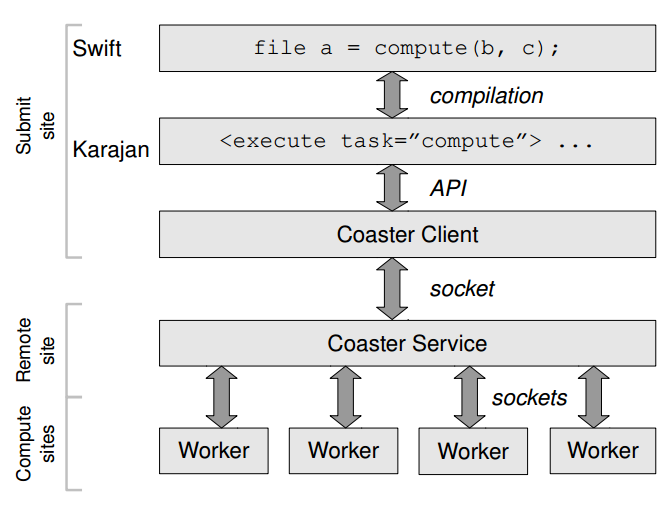
\includegraphics[width=0.8\linewidth,keepaspectratio]{swift/coasters.png}

        There are also several methods of file staging that can be used. This includes a \textit{proxy} mode, which allows files to be accessed from the client side and is delivered to the remote site through the coasters protocol. Another mode available is \textit{file} mode, where the files are on some node remote from the client, but available to the remote Coaster service. Lastly, the \textit{shared file system (SFS)} mode uses a file system that is directly accessible to the Coaster worker node and can be adjusted using standard OS mechanisms.

        In general, Coasters performs fairly well against general methods of job submissions, having low run times between parallel jobs and lower run times for sequential jobs than SSH. With higher numbers, they find average job runtimes on their test system was ~15 seconds. In this case, the job was a protein-RNA docking application.

\subsection{Configuration}

    A site may be configured with Swift using a configuration file, typically named \textit{swift.conf}. It is typically created using a JSON format, although commas are optional if there is a newline and : or = can be used for assigning values. Comments can also be added using // or \#. You can include other configuration files by using the \texttt{include} keyword followed by a string containing the absolute path to the file. Properties (JSON Objects) can also be merged if they have the same name with different keywords. If any collisions occur (same parameters) the later defined one is chosen.

    A Swift configuration file contains the site declarations, global application declarations, and any Swift configuration properties to be defined. This can also include site selection, which is an array of site names as strings. A typical site declaration looks similar to the JSON below:
    \begin{lstlisting}[language=swift]
site.<name> {
    execution {...}
    [staging: "swift" |
        "local" | "service-local" |
        "shared-fs" | "wrapper"]
    [filesystem {...}]
    workDirectory: <path>

    [<site options>]
    [<application declarations>]
}

sites: ["site1", "site2"]
    \end{lstlisting}
    Which define what is used for staging, the work directory, as well as site options and optional app declarations used to define specifics for given app procedures. This can include, the executable, the job queue mechanism, the job project mechanism, and the max execution time (referred to as max wall time).

    Another property, execution, gives Swift information for how applications should be executed on a site. This includes type, or what form of execution should be used with Swift. Such options include local, coasters, SSH, and other typical remote options for Swift. You may also define the job manager, as well as options such as max number of jobs, tasks per node, and other misc options used for debugging. More information on configuration can be found in the User Guide \cite{website:swift-lang-user-guide}.

\subsection{Runtime Environment}

    Swift's runtime system has three reliability mechanisms that are used to handle errors in execution, \textit{retries}, \textit{restarts}, and \textit{replication}.\cite{wilde2011swift} Its first mechanism, \textit{retries}, simply allows Swift to rerun the program. In this case, it is a complete reattempt, starting with site selection, to stage-in, then execution, and finally stage-out. This is strong method is the simplest way of dealing with possible network errors or transient errors that could have occurred. However, if there is an actual bug in the application program then the retry will fail. For this case, Swift keeps a \textit{restart log} so that a later run may start with this log and avoid re-executing other applications that may have been successful.

    However, another form of failure can occur, which is an extended time of being enqueued on a site. In this case, the site has failed because it will either take an extended amount of time til it can run (\textit{soft failure}) or it was running at some point and halted the process jobs or all processing in general (\textit{hard failure}). To deal with issue, Swift uses \textit{job replication}, where a clone of the job is submitted independently with the previous job being canceled.

    However, job submissions can dominate execution time due to congested queues or extended job lengths. To avoid this, Swift gives us two options that we can use, \textit{clustering} and \textit{Coasters}. Coasters we have previously discussed in Section \ref{sec:coasters}, but clustering is more general. Clustering aggregates multiple program executions into a single job, which in turn reduces the number of job submissions. This method requires an estimate on the number of available remote nodes and job duration in order to pick a reasonable cluster size. If this estimate is incorrect, the site may have an insufficient number of worker nodes or an excessive number of job submissions. However, Coasters is more dynamic and allows for queueing and execution in more parallel systems, allowing for more work to be done beforehand.

    There can be difficulty in using Swift for a large number of sites, as a basic site catalog isn't practical. This is due to the variations that can exist from site to site and the possibility of user applications not being installed on a given site. However, catalogs are more straightforward, leading Swift to be interfaced with site catalog that is generated from another system. This catalog scores different sites to deal with the majority of situations, but new failure conditions can arise, leading the necessity of Swift to develop more robust fault tolerance mechanisms to fix these site issues. As for missing user applications, they are compiled statically and sent as a small number of self-contained files. Swift then uses its existing input file management system to stage the application files once per site per run.

\subsection{Applications}

    As we can tell from the previous sections, Swift isn't a language used in most common applications such as C/C++, Java, or Python. Instead, its use of single-assignment variables and focus on execution timing and remote site distribution paints a different, primarily used for scientific programming and adjusting frameworks. We can see this in many applications and systems that use Swift, such as high-resolution climate data analysis \cite{woitaszek2011parallel}, protein folding, petascale data management and scripting \cite{wilde2009parallel}, as well as other general applications in thermodynamics and image data processing \cite{wilde2011swift}.

    Climate data can be incredibly large, especially when dealing with large time spans. To analyze 10-years of atmospheric data can take over 90 minutes on an 8-core node. However, with the use of Swift this processing can be decreased to about 30 minutes and less as more nodes are used for processing. This is due to not only the large amount of data being used, but also how frequently it is used for other processes. In this case, the use of Swift aids in the construction of several models used for climate statistic analysis, each of which using several gigabytes of information for each part of processing \cite{woitaszek2011parallel}. Because we are able to prepare for later applications as well as better time our jobs within our queues, Swift can cut our time dramatically.

    We can also see this application for protein folding \cite{wilde2009parallel}, as Swift can increase the parallelization for several jobs, thereby allowing more structures to be generated in a smaller amount of time. In this case 67,178 structure predictions were discovered in 2 weeks, or approximately 200 structures predicted per hour. It has also been used for computing 100,000 Monte Carlo glass cavity simulations, which is used for understanding thermodynamics. This has also been thought of as a case study to explore peta-scale scripting, which is a fairly open field for next-gen computation.

\subsection{Performance}

    As stated before, resultings using climate data analysis \cite{woitaszek2011parallel} has shown vast improvements by switching to Swift, cutting times down by a third with a single node. We also see improved results when comparing the Coasters framework using Swift with an SSH framework, cutting times down significantly when testing with protein folding. This also corresponds with the protein folding case study which generated a significantly amount of predicted structures \cite{wilde2009parallel}.

    Swift also keeps utilization of processes high, sustaining 100 concurrent application at 90\% CPU utilization and 85\% with 200 concurrent applications. When using a node-based system, we can see even better results with tasks lasting at least 100 seconds with several nodes having a utilization of 95\% and tasks with lower duration given less utilization.

\subsection{Our Experience}

    For our programming project, our group tasked ourselves with a basic concurrent programming script, matrix multiplication. Although this is more reasonable within other languages, it feels almost impossible with Swift. This is due to how Swift has single-assignment variables and relies heavily on other applications, as its main purpose is to aid in overall job performance. In order to do matrix multiplication with Swift, you have to have some program read the entire matrix then do the threading on its own, rendering Swift useless in this instance. Although Swift is useful for job management and large grid computing, it certainly doesn't work well for basic programs such as matrix multiplication.

    We also found it difficult to find any aid on Swift, which is worsen by Apple's choice of creating a new iOS programming language also called Swift with the same bird representing their language. Even typing "swift concurrent" or "swift-lang" or any particular key phrases for our Swift would lead to some article, blog, or discussion on Apple's Swift, forcing us to back-trace or look deeper through the material. It is also difficult to debug due to this, as you could have issues in other applications or Swift which could be mentioned through the JVM, making it more difficult to read error messages.
